\section{Künstliche neuronale Netze}

\begin{slide}{Künstliche neuronale Netze}
	\begin{itemize}
		\item Zweig der künstlichen Intelligenz
		\item nach biologischem Vorbild
		\item Netz aus "Neuronen"
		\item liefert Ausgabewert zu Eingaben
		\item kann von Beispielen lernen
	\end{itemize}
	\begin{center}
		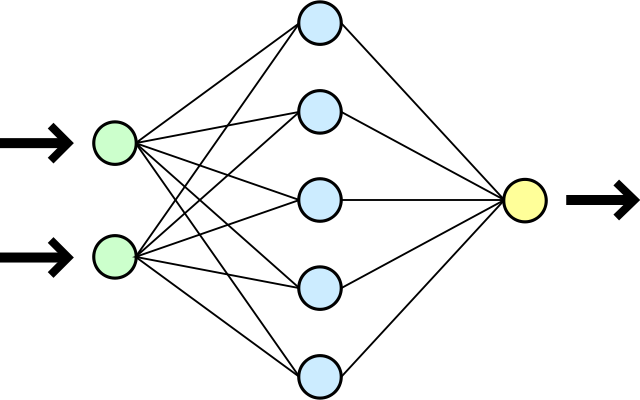
\includegraphics[width=\textwidth,height=0.4\textheight,keepaspectratio]{content/Neural_network}
	\end{center}
\end{slide}

\begin{slide}{Neuron}
	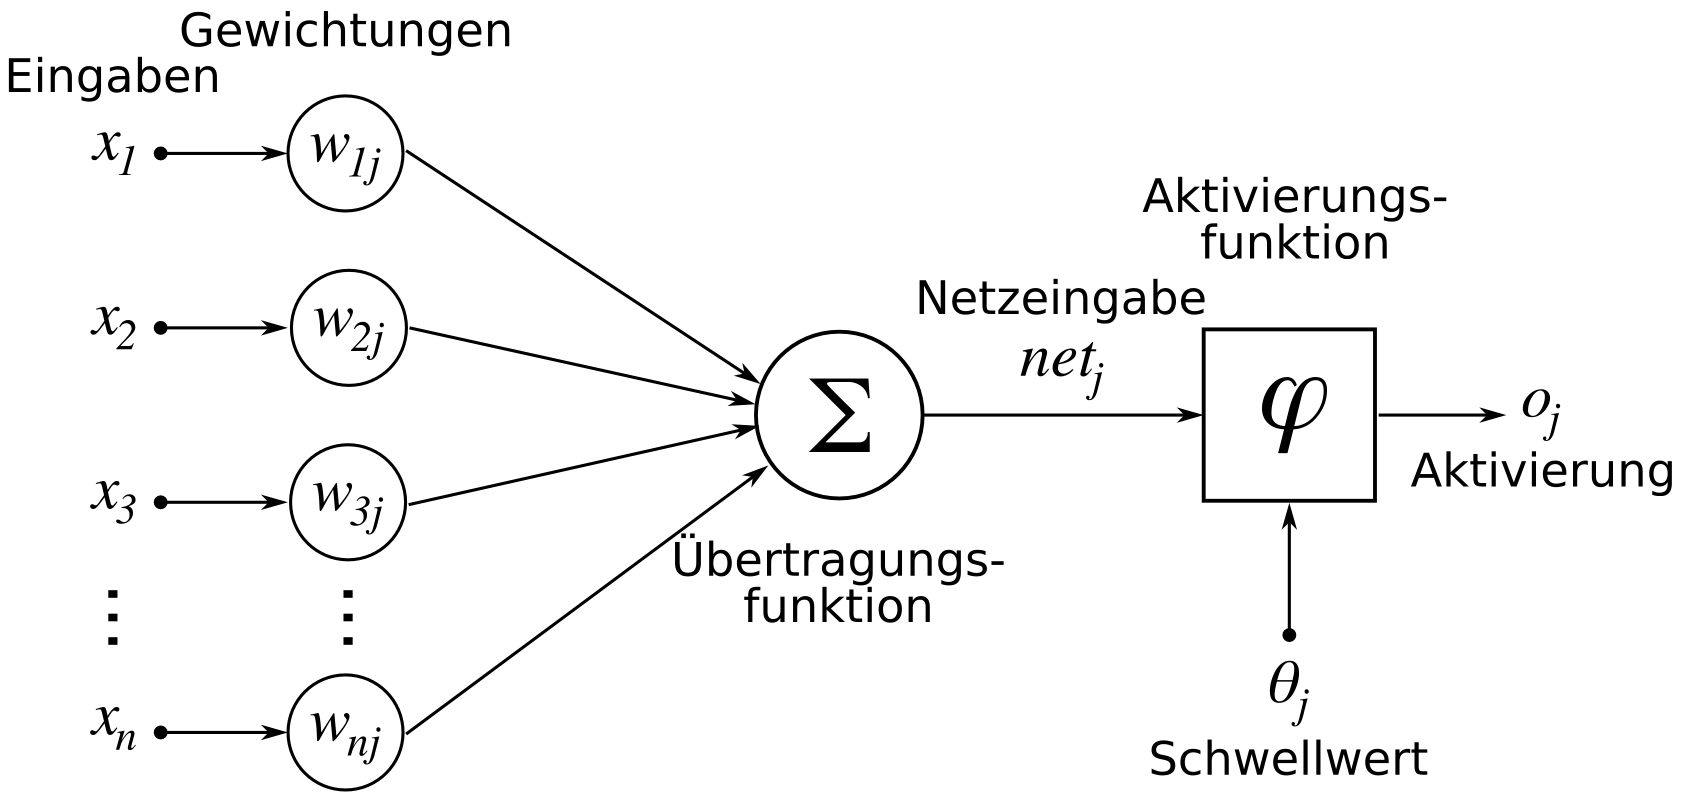
\includegraphics[width=\textwidth,height=0.8\textheight,keepaspectratio]{content/ArtificialNeuronModel}
	\blfootnote{„ArtificialNeuronModel deutsch“ von Chrislb. Lizenziert unter CC BY-SA 3.0 über Wikimedia Commons}
\end{slide}

\begin{slide}{Netzwerk}
	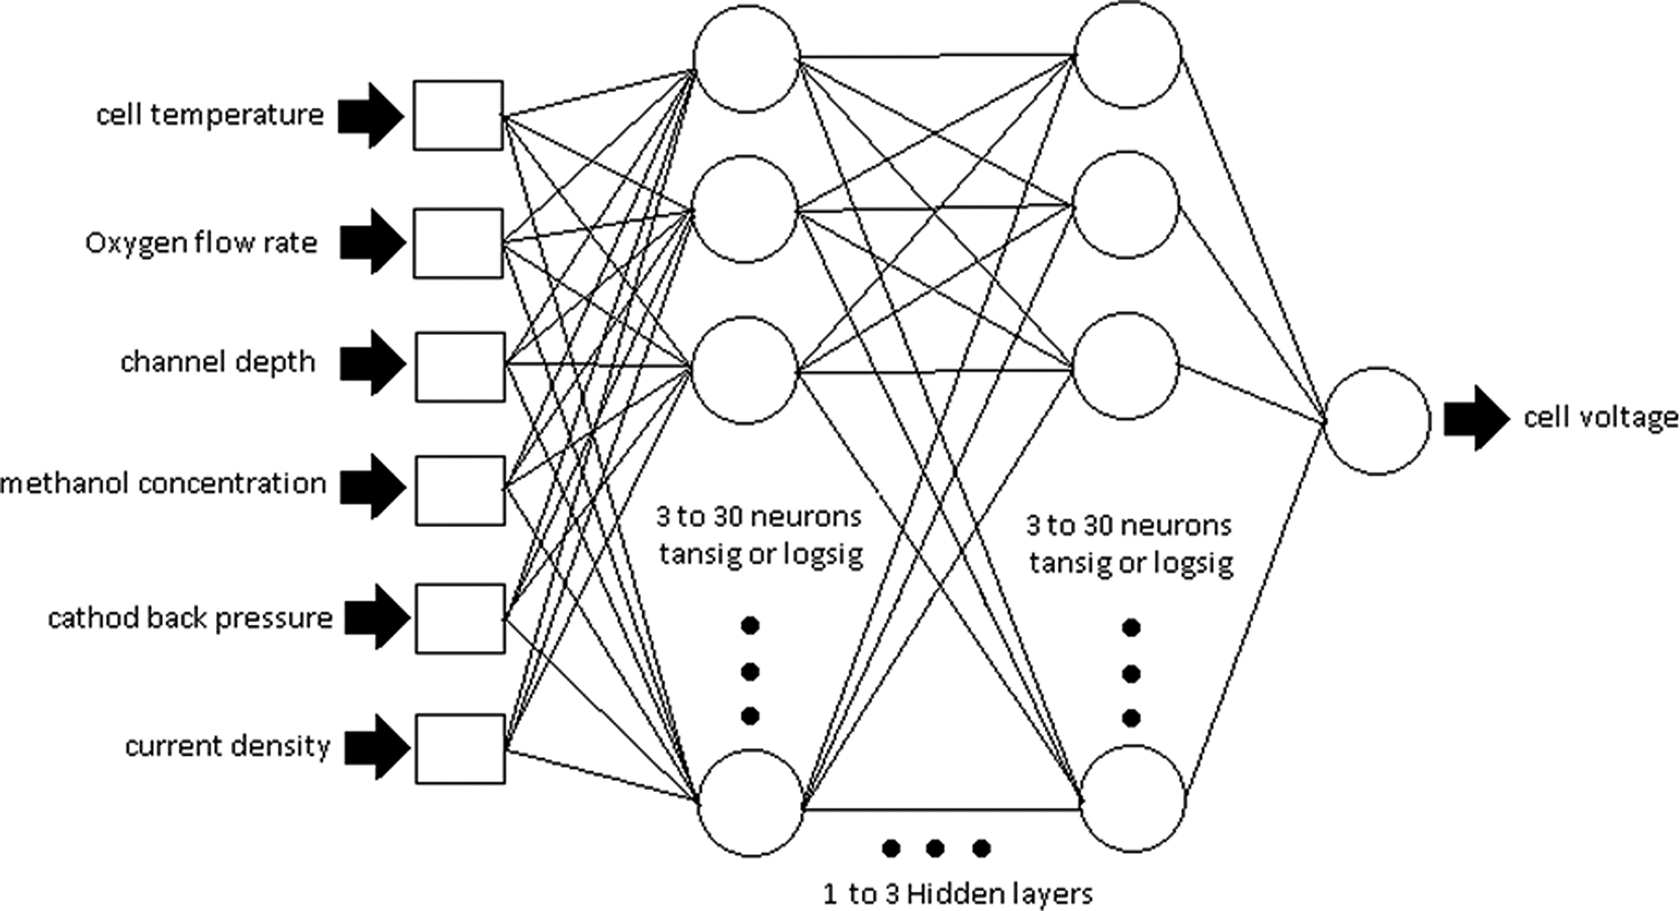
\includegraphics[width=\textwidth,height=0.8\textheight,keepaspectratio]{content/knn_fuel}
	\blfootnote{Tafazoli M, Baseri H, Alizadeh E, Shakeri M. Modeling of Direct Methanol Fuel Cell Using the Artificial Neural Network. ASME. J. Fuel Cell Sci. Technol. 2013}
\end{slide}

\begin{slide}{Künstliche neuronale Netze}
	\begin{itemize}
		\item lernen durch anpassen von Gewichten
		\item verschiedene Lernalgorithmen
		\item anlernen von Eingabe-Ausgabe-Paaren
	\end{itemize}
\end{slide}


\begin{slide}{Anwendung}
	Besonders geeignet wenn wenig systematisch nutzbares Wissen vorliegt.
	\begin{itemize}
		\item Texterkennung
		\item Bilderkennung
		\item Gesichtserkennung
		\item Prognosen
		\item Frühwarnsysteme
		\item KI in Spielen und Simulationen
	\end{itemize}
\end{slide}
